%%
%% Elsevier elsarticle template. Build with:  latexmk -pdf document.tex
%%
\documentclass[preprint,12pt]{elsarticle}

\usepackage{amsmath}
\usepackage{amssymb}
\usepackage{dsfont}
\usepackage{booktabs}
\usepackage{longtable}
\usepackage{url}
\usepackage{algorithm}
\usepackage{algpseudocode}
\usepackage{xcolor}
\usepackage[hidelinks]{hyperref}

\newcommand{\code}[1]{\texttt{#1}}

\newtheorem{remark}{Remark}

%\journal{}

\begin{document}
\begin{frontmatter}

\title{\textbf{American Airlines COMPASS Competition, Fall 2026}\\Flight Dispatcher Annual Workforce Planning:\\ An Exact Bid-line and Shrinkage Model for Phases I and II}

\affiliation[1]{The COMPASS Predictive Hokies}
\affiliation[2]{Grado Department of Industrial and Systems Engineering, Virginia Tech, Blacksburg, Virginia 24060, USA}
\affiliation[3]{Department of Computer Science, Virginia Tech, Blacksburg, Virginia 24060, USA}
\author[1,2]{Akshat Kothyari}
\author[1,2]{Daniel Neira}
\author[1,3]{Jiayi Xue}

\begin{abstract}
   American Airlines plans its flight-dispatcher workforce a full year ahead, deciding how many bid lines to create across eight work centers and three shifts and how to schedule them so that every desk is staffed without carrying unnecessary staff. Phase I poses the pure bid-line covering problem. Phase II adds \emph{shrinkage}: mandatory training and vacation that consume scheduled working days, together with the rules that govern it. We report a two-part solution. For Phase I we exploit the exact separability of the problem into independent work-center/shift covering model and solve the small integer programs exactly. For Phase II, we observed that the only couplings introduced are per-day shared capacities (the 12-seat training class and the daily vacation quota) adding to the addition of possible flex days. We build an exact mixed-integer model that places each mandatory training day where it does least damage to coverage. The training model decomposes, without loss, into one small program per (shift, month) pair, which is solved using Gurobi and Xpress solvers. On the competition instance the exact training layer reduces under-coverage from 4,417 to 4,221 seat-days and surplus supply from 6,050 to 5,861 relative to a random placement.
\end{abstract}

%\begin{keyword}
%   \sep
%\end{keyword}

\end{frontmatter}

% ========================================================================== %
\section{Introduction}
% ========================================================================== %
American Airlines operates nearly 6,800 flights per day, each coordinated from its Integrated Operations Center (IOC) by a flight dispatcher who shares legal responsibility with the captain for the safety of the flight. Dispatchers must be on duty across a 24-hour operation every day of the year. The workforce is therefore planned a full year ahead: the plan decides how many \emph{bid lines} (pre-built annual work schedules) to create and how to schedule them so that demand is covered as closely as possible without carrying surplus staff.

The competition releases the problem in two phases. Phase I is the core scheduling problem: given daily desk demand across eight work centers and three shifts, decide how many bid lines to create and at which offsets to place them. Phase II adds \emph{shrinkage}: mandatory training and vacation remove scheduled working days, flex days add them, and a set of rules governs where each may fall.

This manuscript documents the model we implemented:
\begin{enumerate}
   \item for Phase I, we exploit the exact separability of the problem into independent work-center/shift covering models, which decomposes into 24 independent cyclic-covering problems, for this small problems an exact integer model is implemented;
   \item an exact Phase II training model that chooses training days to minimize coverage damage subject to the mandatory-training, one-per-day and shared class-size rules, with a lossless decomposition into (shift, month) programs.
\end{enumerate}

The notation used throughout is collected in Table~\ref{tab:notation} of Appendix~\ref{app:notation}, grouped into sets and indices, parameters, and decision variables.

% ========================================================================== %
\section{Problem description}
% ========================================================================== %
   \subsection{Phase I: bid lines and coverage}
      The planning year runs 14 January 2025 through 11 January 2026 (363 days, $24\times15+3$ cycle lengths). A \emph{desk} is a staffed position; one dispatcher works one desk for one shift. Demand is given per combination of calendar day, work center and shift: the instance contains 8,664 such coverage obligations totaling 82,252 required desk-days. Dispatchers are organized into eight work centers, four geographic (Domestic, Latin, Europe, Pacific) and four specialized (ATC, ROC, CHF, OC) as shown in Table~\ref{tab:work_centers}, across three 8-hour shifts (MORNING, EVENING, MIDNIGHT) as shown in Table~\ref{tab:shifts}, giving 24 work-center/shift combinations. Domestic alone accounts for roughly half of demand.

      \begin{table}[h!]
         \centering
         \caption{Work Centers}
            \begin{tabular}{ll}
            \toprule
            Group & Work Centers \\
            \midrule
            Geographic regions & Domestic, Latin, Europe, Pacific \\
            Specialized centers & ATC, ROC, CHF, OC \\
            \bottomrule
            \end{tabular}%
         \label{tab:work_centers}%
      \end{table}%

      \begin{table}[h!]
      \centering
      \caption{Shifts}
         \begin{tabular}{lll}
         \toprule
         Shift &  Start & End \\
         \midrule
         MORNING  & 5:00  & 13:00 \\
         EVENING  & 13:00 & 21:00 \\
         MIDNIGHT  & 21:00 & 05:00 \tiny{(next day)}\\
         \bottomrule
         \end{tabular}%
      \label{tab:shifts}%
      \end{table}%

      A bid line is created for one work center and one shift and keeps both all year. Every bid line follows the FAA 4-3-4-4 pattern over a repeating 15-day cycle ($[1,1,1,1,0,0,0,1,1,1,1,0,0,0,0]$): four days on, three off, four on, four off. The pattern is fixed; lines differ only by their \emph{offset}, that is, where in the cycle they start, of which there are 15. A bid line thus works 8 of every 15 days, and which calendar days it covers is fixed by its offset. A bid line may also receive up to four \emph{flex days}, converting scheduled days off into working days. A graphic view on the 15 possible offsets is shown in Figure~\ref{fig:offset}, and similarly the three possible shifts are shown in Figure~\ref{fig:shifts}.
      
      \begin{figure}[h!]
         \centering
         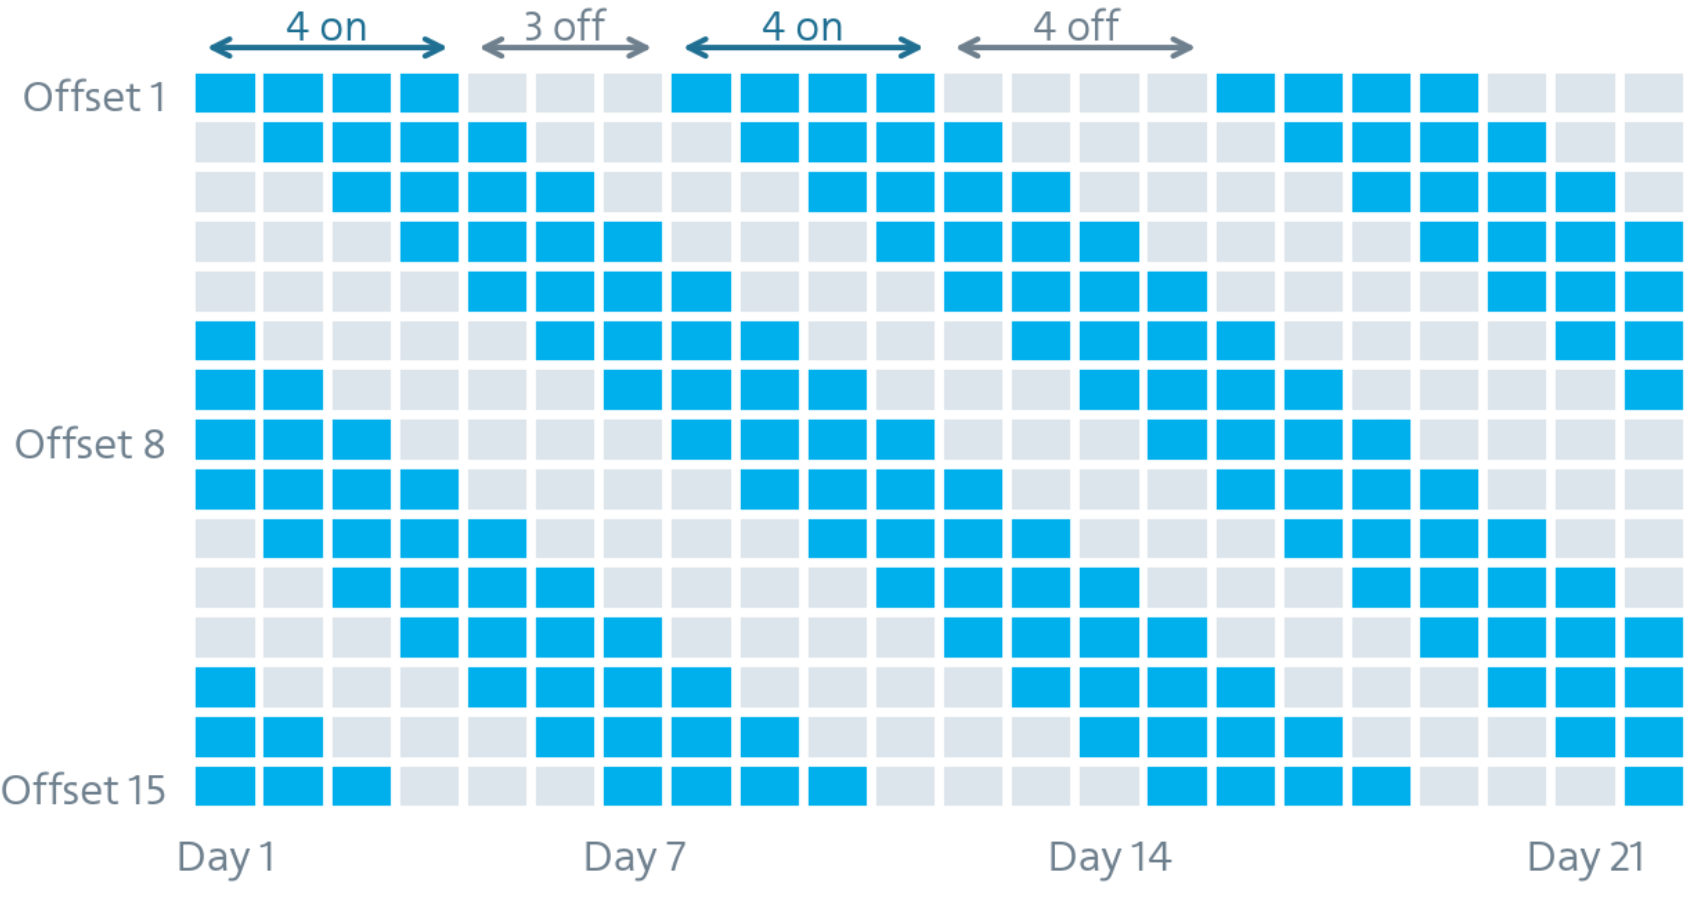
\includegraphics[width=0.7\linewidth]{figs/offset.png}
         \caption{All 15 possible offsets: the same 15-day cycle, each starting one day later}
         \label{fig:offset}
      \end{figure}

      \begin{figure}[h!]
         \centering
         
\includegraphics[width=0.5\linewidth]{figs/shifts.png}
         \caption{3 possible shifts: morning, afternoon, and midnight}
         \label{fig:shifts}
      \end{figure}

      Coverage is assessed per (day, work center, shift), and a bid line contributes only to its own work center and shift. The stated optimization goals, in priority order, are: (1) close staffing gaps (under-coverage), (2) use as few bid lines as possible, and (3) avoid coverage beyond demand (over-coverage).

   \subsection{Phase II: shrinkage}
      Phase II introduces three rules that change what a scheduled day actually does: \emph{vacation} turns a working day into one that covers nothing; \emph{training} does the same; \emph{flex days} turn a day off into a working day. A day can do only one job: a flex day cannot also be a training or vacation day, and training and vacation cannot coincide.

      \paragraph{Vacation} Vacation is an entitlement allocated as a number of dispatchers per calendar day: a base of 27 plus or minus up to 2, so between 25 and 29 dispatchers per day. The adjustment is set inversely to daily operational volume, so quieter days carry more vacation. Vacation falls only on a scheduled working day, not on a flex day, and not on a training day. Both across-line and across-year balance matter.

      \paragraph{Secondary qualifications} A bid line's work center determines its primary qualification; every line also holds Domestic; beyond that, secondary qualifications may be assigned. Each secondary qualification held requires its own training, so more qualifications mean more shrinkage. The competition permits any assignment method, and we implement the supplied three-step pseudocode (map lines to historical records, estimate co-occurrence proportions, sample secondaries in those proportions) \citep{compasspseudo}.

      \paragraph{Training} Training is mandatory. Every bid line trains for Domestic and for each qualification it holds beyond Domestic, once in each of that qualification's designated months (as shown in Table~\ref{tab:qualifications_elegible_training_months}). Training falls only on a scheduled working day, not on a flex or vacation day, and at most once per line per day. Training capacity is limited by a \emph{class size} of 12 per shift per day, counted across \emph{all} work centers: work centers compete for the same seats.

      \begin{table}[h!]
         \centering
         \caption{Eligible training months for each qualification}
         \begin{tabular}{ll}
         \toprule
         Qualification & Eligible months \\
         \midrule
         Domestic  & February, May, September \\
         Europe & March \\
         Pacific & April \\
         Latin & October \\
         ATC   & March, November \\
         ROC   & October \\
         CHF   & October \\
         OC    & March \\
         \bottomrule
         \end{tabular}%
         \label{tab:qualifications_elegible_training_months}%
      \end{table}%

      All this new features adds complexity to the scheduling process, they are summarized in Figure~\ref{fig:phase_ii}.
      \begin{figure}[h!]
         \centering
         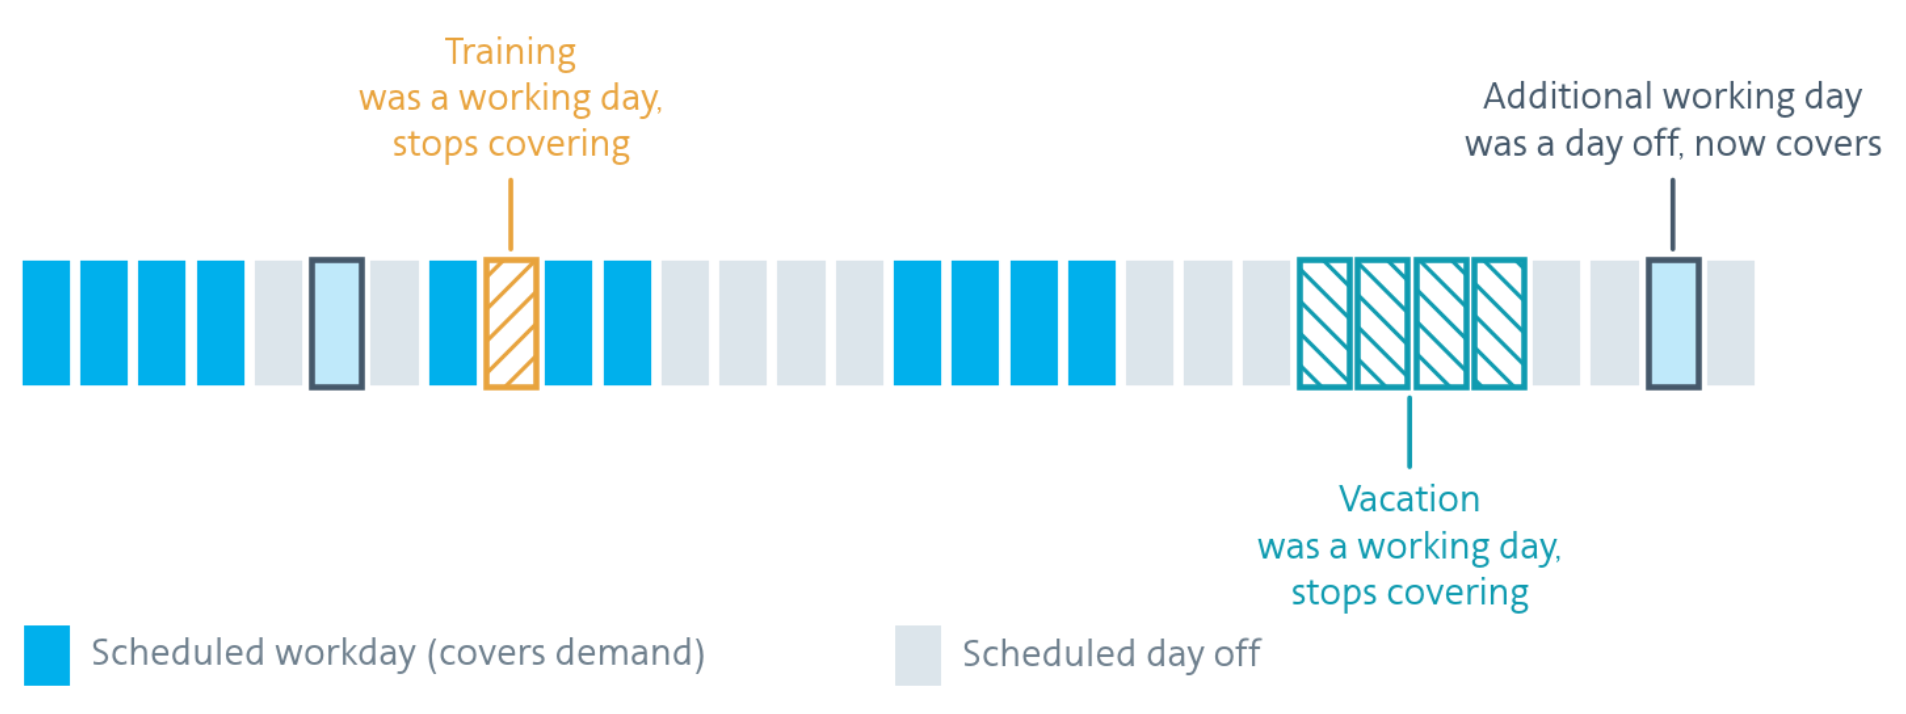
\includegraphics[width=0.9\linewidth]{figs/phase_ii.png}
         \caption{Vacation and training remove coverage, an additional working day adds it}
         \label{fig:phase_ii}
      \end{figure}

% ========================================================================== %
\section{Brief literature review}\label{sec:lit}
% ========================================================================== %
   This work sits between personnel scheduling, cyclic days-off scheduling, and airline crew scheduling. The reviews of Ernst et al. \citep{ernst2004staff}, Van den Bergh et al. \citep{vandenbergh2013personnel}, and Alfares \citep{alfares2004survey} map the field: demand modeling, days-off assignment, shift assignment, and tour scheduling, including the compressed workweeks and cyclic patterns used here. The bid-line covering model for Phase I is a cyclic days-off model in the sense of Baker \citep{baker1974scheduling}; for the two-shift case its constraint matrix has the circular-ones property and the LP relaxation is integral \citep{bartholdi1980cyclic}, with a guaranteed-accuracy rounding scheme when it is not \citep{bartholdi1981roundoff}.

   Airline workforce planning is the closest application. Holloran and Byrn \citep{holloran1986united} report a deployed station manpower and bid-line system, and Barnhart et al. \citep{barnhart2003applications} and Gopalakrishnan and Johnson \citep{gopalakrishnan2005airline} survey crew scheduling, where set-covering and set-partitioning formulations solved by column generation are standard \citep{dantzig1960decomposition,vance1997airline,desaulniers2005column,irnich2005shortest}; the lineage starts with Dantzig's set-covering formulation \citep{dantzig1954comment} and early set-partitioning work on vehicle scheduling \citep{foster1976integer}.

   On the objective and the shrinkage layer, mixed-integer staff scheduling is well studied \citep{beaumont1997scheduling}, excess off-days and idle time are modeled explicitly by \"Ozg\"uven and Sungur \citep{ozguven2013integer}, and days-off preferences are handled by goal programming in Shuib and Kamarudin \citep{shuib2018solving}. Flexible intra-tour choices can be modeled implicitly rather than by enumerating every pattern \citep{bechtold1990implicit}, and annualized hours frame the value of extra working days across a year \citep{corominas2005annualised}. Planning a year ahead against uncertain shrinkage is a robustness problem, for which the budget-of-uncertainty approach of Bertsimas and Sim \citep{bertsimas2004price} is a tractable route.

% ========================================================================== %
\section{Data exploration and diagnostics}
% ========================================================================== %
   \paragraph{Demand} The instance has 363 distinct dates, 24 work-center/shift combinations and 8,664 demand rows totaling 82,252 desk-days. Demand per row ranges from 1 to 52 with median 6; it varies across the year and the day of week. One work center (Domestic) contributes about 50\% of all demand as shown in Figure~\ref{fig:daily_demand_per_wc}.
   
   \begin{figure}[h!]
      \centering
      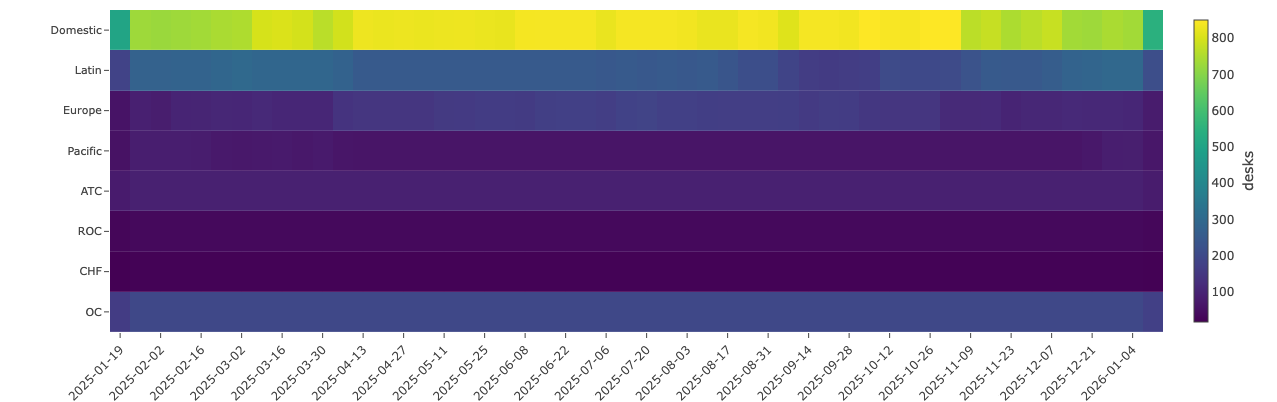
\includegraphics[width=1\linewidth]{figs/daily_desk_demand_per_wc.png}
      \caption{Daily desk demand by work center and shift (14 Jan 2025 - 11 Jan 2026)}
      \label{fig:daily_demand_per_wc}
   \end{figure}

% ========================================================================== %
\section{Phase I methodology}
% ========================================================================== %
   \subsection{Separability and the offset-covering structure}
      A bid line is fixed to one work center and one shift, and coverage constraints never couple two work centers. The Phase I problem therefore decomposes into 24 independent subproblems, one per work-center/shift combination. Within a subproblem the only real decision is how many bid lines to create at each of the 15 offsets. With $n_\kappa$ the number of lines created at offset $\kappa$ ($\kappa \in \{0,\ldots,14\}$) and $\alpha_{\kappa\delta}\in\{0,1\}$ indicating whether offset $\kappa$ works cycle position $\delta$ ($\delta \in \{0,\ldots,14\}$), the base model is the integer program
      \begin{equation}
         \min \; \sum\limits_{\kappa=0}^{14} n_\kappa
         \quad\text{s.t.}\quad
         \sum\limits_{\kappa} \alpha_{\kappa\delta}\,n_\kappa \;\ge\; D_\delta \;\;\quad \forall \delta,
         \qquad n_\kappa \in \mathbb{Z}_{\ge 0},
         \label{eq:phase1}
      \end{equation}
      a cyclic covering problem of the classical days-off/tour-scheduling family \citep{baker1974scheduling,alfares2004survey,ernst2004staff}. We enumerate the offset vectors directly rather than encode the cycle as constraints, so the model contains only 15 integer variables per subproblem.

% ========================================================================== %
\section{Phase II methodology}
% ========================================================================== %
   The Phase II rules introduce only two per-day shared capacities: the training class of 12 seats per (day, shift) across all work centers, and the daily vacation quota of 25 to 29 dispatchers across all shifts and work centers. The daily demand, the offset calendar, and the working-day restriction all stay per-slot, which shapes the model below.

   \subsection{Qualification assignment}
   We implement the supplied three-step pseudocode: rank historical employees by qualification breadth and map them onto bid lines; build the historical co-occurrence table $P(\text{holds }y \mid \text{primary}=x)$; and sample secondary qualifications in those proportions. The resulting qualification mix fixes the training load and hence the shrinkage. This stage is preprocessing and does not enter the optimization; the full pseudocode is given as Algorithms~\ref{alg:map}--\ref{alg:sprinkle} in Appendix~\ref{app:quals}. The corresponding table with values to match (proportion) is shown below in Table~\ref{tab:prevalence_primary_secondary_quals}.

   \begin{table}[h!]
      \centering
      \caption{Prevalence of primary/secundary qualifications}
      \begin{tabular}{c|ccccccc}
      \toprule
      Primary\textbackslash{}Secundary & ATC   & ROC   & CHF   & OC    & Latin & Europe & Pacific \\
      \midrule
      ATC   & -     & 0.16  & 0.4   & 0.44  & 0.2   & 0.08  & 0.08 \\
      ROC   & 0.2   & -     & 0.3   & 0.5   & 0.4   & 0.2   & 0.2 \\
      CHF   & 0.5   & 0.33  & -     & 0.33  & 0.67  & 0.5   & 0.5 \\
      OC    & 0.35  & 0.2   & 0.24  & -     & 0.3   & 0.11  & 0.13 \\
      Latin & 0.04  & 0.02  & 0.06  & 0.09  & -     & 0.17  & 0.24 \\
      Europe & 0.02  & 0.02  & 0.02  & 0.06  & 0.25  & -     & 0.56 \\
      Pacific & 0.07  & 0.03  & 0.07  & 0.03  & 0.1   & 0.79  & - \\
      \bottomrule
      \end{tabular}%
      \label{tab:prevalence_primary_secondary_quals}%
   \end{table}%

   \subsection{Exact training placement}
   Let $r=(\ell,q,m)$ be the requirement that bid line $\ell$ trains for qualification $q$ in month $m$, and let $E_r$ be the set of dates bid line $\ell$ is scheduled to work in month $m$ (\emph{excluding flex and vacation dates}). Let $y_{rt}$ be the binary variable indicating whether requirement $r$ is scheduled for training on date $t$, and let $z_{wt}$ be the number of training days removed from slot $(w,t)$, where $w$ is a work center and $t$ a date; let $\beta_{wt}$ and $D_{wt}$ be the roster supply and demand on that slot. We solve, per shift $s$, the model
   \begin{align}
      \min \;\; & p^{under}\sum\limits_{w,t} u_{wt} \;+\; p^{surplus}\sum\limits_{w,t} o_{wt} \label{eq:mod1:obj}\\
      \text{s.t.}\;\; & \sum\limits_{t\in E_r} y_{rt} = 1 && \forall r \label{eq:mod1:con1}\\
      & \sum\limits_{r:\,\ell(r)=\ell,\;m(r)=m} y_{rt} \le 1 && \forall \ell,m,t \label{eq:mod1:con2}\\
      & \sum\limits_{r:\,\text{shift}(r)=s} y_{rt} \le C^{size} && \forall t \label{eq:mod1:con3}\\
      & z_{wt} = \sum\limits_{r} y_{rt} \cdot \mathds{1}_{[\ell(r)\in w]} && \forall w,t \label{eq:mod1:con4}\\
      & u_{wt} \ge D_{wt} - (\beta_{wt}-z_{wt}),\quad o_{wt} \ge (\beta_{wt}-z_{wt}) - D_{wt} && \forall w,t \label{eq:mod1:con5}\\
      & z_{wt}\in\mathbb{Z},\quad u_{wt},o_{wt}\ge 0  && \forall w,t \label{eq:mod1:con6} \\
      & y_{rt}\in\{0,1\},  && \forall r,t. \label{eq:mod1:con7}
   \end{align}
   
   The objective function \eqref{eq:mod1:obj} meets the demand by minimizing weighted coverage penalties: under-coverage penalty $p^{under}$ and a surplus (over-coverage) penalty $p^{surplus}$ are used to penalize deviations from the desired coverage levels. 
   Constraint \eqref{eq:mod1:con1} schedules each requirement $r$ exactly once, on one of the dates the bid line works that month. 
   Constraint \eqref{eq:mod1:con2} allows at most one training per bid line per date, so two qualifications of the same bid line that share a month cannot fall on the same date. 
   Constraint \eqref{eq:mod1:con3} limits trainees to $C^{size}$ per (date, shift) across all work centers, the only constraint that couples work centers. 
   Constraint \eqref{eq:mod1:con4} defines $z_{wt}$ as the number of trainings removed from slot $(w,t)$, where $\mathds{1}_{\ell(r)\in w}$ is the indicator function for the event that bid line $r$ is in work center $w$; and constraint \eqref{eq:mod1:con5} turns those removals into under-coverage $u_{wt}$ and over-coverage $o_{wt}$ relative to the roster supply $\beta_{wt}$ and the demand $D_{wt}$. 
   Constraint \eqref{eq:mod1:con6} imposes integrality on $z_{wt}$ and nonnegativity on $u_{wt}$ and $o_{wt}$, and constraint \eqref{eq:mod1:con7} fixes $y_{rt}$ as binary.

   The penalties $p^{under}$ and $p^{surplus}$ mirror the evaluator's asymmetric treatment of under-coverage and surplus. 
   %Because $z_{wt}$ is integer in \eqref{eq:mod1:con4} and the coverage terms in \eqref{eq:mod1:con5} make the objective convex, \eqref{eq:mod1:obj} is an exact convex-cost assignment program: training is pushed onto slack-rich, low-demand days and away from cells that are already tight. 
   %This objective mirrors the explicit treatment of excess off-days and idle time in the scheduling literature (Section~\ref{sec:lit}).

   \begin{remark}[Lossless (shift, month) decomposition] 
      Training months never share calendar dates. The class cap, the per-bid-line-per-day rule, and coverage are all per-date constraints, so nothing couples two months and the union of the per-(shift, month) optima is the global optimum. We solve one program per (shift, month) pair.
   \end{remark}

% ========================================================================== %
\section{Vacation: rules, quota and assignment}
% ========================================================================== %
   Vacation is an \emph{entitlement}: the number of dispatchers on vacation on each calendar day is fixed and cannot be optimized away. Only \emph{where} the vacation falls is ours to decide, and the plan must absorb it.

   \subsection{Rules as constraints}
   Let $\mathcal{T}$ be the set of calendar dates in the planning year and, for each line $\ell$, let $R_\ell$ be the set of dates it is scheduled to work under its bid-line offset and $\bar{R_\ell}$ its complement (the dates it is not scheduled to work); and $F_\ell$ its (possibly empty) flex dates. The assignment variables $\nu_{\ell t}\in\{0,1\}$, where line $\ell$ is on vacation on date $t$, must satisfy
   \begin{align}
      & \sum\limits_{\ell} \nu_{\ell t} \;=\; Q_t && \forall t \in \mathcal{T} \label{eq:mod2:con1}\\
      & \nu_{\ell t} = 0 && \forall \ell,\; t \in \bar{R_\ell} \label{eq:mod2:con2}\\
      & \nu_{\ell t} = 0 && \forall \ell,\; t \in F_\ell \label{eq:mod2:con3}\\
      & \nu_{\ell t} + \tau_{\ell t} \le 1 && \forall \ell, t \label{eq:mod2:con4}
   \end{align}
   where $Q_t\in\{25,\dots,29\}$ is the date's quota and $\tau_{\ell t}\in\{0,1\}$ marks a training date. Constraint \eqref{eq:mod2:con1} sets the daily vacation count to exactly $Q_t$; it is an equality, not a bound, so the quota must be met. Constraint \eqref{eq:mod2:con2} allows vacation only on dates the line is scheduled to work. Constraint \eqref{eq:mod2:con3} forbids vacation on a flex date. Constraint \eqref{eq:mod2:con4} forbids vacation on a date the line trains, using the training indicator from \eqref{eq:mod1:obj}. Training is scheduled \emph{before} vacation, so the no-overlap rule is enforced by removing training days from the pool of eligible vacation days.

   Two balance requirements accompany the hard rules, both assessed by the metrics of Section~\ref{sec:metrics}: across bid lines, vacation should be proportional so no line absorbs a disproportionate share; across the year, it should be spread so coverage is not disrupted in particular months, weeks or days.

   \subsection{Daily quota from operational volume}
   Busyness is measured by the unitless operational volume $\eta_t$ in the reference volume file, which is \emph{not} desk demand. We rank the dates by $\eta_t$ and partition the ranking into $2M+1$ bands of near-equal size, with $M=2$ the maximum variable adjustment. Writing $Q_{\text{base}}=27$, a date falling in band $j\in\{0,\dots,2M\}$ receives
   \begin{equation}
      Q_t \;=\; Q_{\text{base}} \;+\; (M - j), \qquad Q_t \in \{25, 26, 27, 28, 29\},
   \end{equation}
   so the quietest band gets $+M$ and the busiest gets $-M$: quieter days carry more vacation. We use rank-based bands rather than the raw scaled value to keep integer adjustments; on the instance the bands contain 72/72/72/73/73 days and the resulting correlation between volume and quota is $\mathrm{corr}(\eta_t, Q_t) = -0.87$, a strong inverse relation as intended. The quota routine is given as Algorithms~\ref{alg:scale}--\ref{alg:alloc}, and the continuous rescaling helper used for reporting is defined in Section~\ref{sec:metrics}.

   \begin{algorithm}[h!]
      \caption{Rescale a series to $[-1,1]$.}
      \label{alg:scale}
      \begin{algorithmic}[1]
      \Function{ScaleToRangeNeg1To1}{series}
      \State $lo \gets \min(series)$; $hi \gets \max(series)$
      \If{$hi = lo$}
         \State \Return $series$ of zeros
      \EndIf
      \State $scaled \gets (series - lo)/(hi - lo)$ \Comment{maps to $[0,1]$}
      \State \Return $2\,scaled - 1$ \Comment{maps to $[-1,1]$}
      \EndFunction
      \end{algorithmic}
   \end{algorithm}

   \begin{algorithm}[h!]
      \caption{Assign integer variable-vacation adjustments by demand rank.}
      \label{alg:bands}
      \begin{algorithmic}[1]
      \Function{AssignVariableVacationDays}{\code{demand\_df}, \code{max\_variable\_days}}
      \State $n \gets$ number of rows
      \State $B \gets 2\cdot\code{max\_variable\_days}+1$
      \State $base \gets \lfloor n/B \rfloor$; $extra \gets n \bmod B$
      \State \code{sorted\_indices} $\gets$ row indices sorted by \code{demand} ascending
      \State $pointer \gets 0$
      \For{$bucket = 0$ to $B-1$}
         \State $size \gets base + 1$ if $bucket < extra$, else $base$ \Comment{use the bucket index, not the element index}
         \State $value \gets bucket - \code{max\_variable\_days}$
         \For{$j = 0$ to $size-1$}
            \If{$pointer \geq n$}
               \State \textbf{break}
            \EndIf
            \State \code{categories}[\code{sorted\_indices}[pointer]] $\gets value$
            \State $pointer \gets pointer + 1$
         \EndFor
      \EndFor
      \State \Return \code{demand\_df} with column \code{variable\_vacation} mapped from \code{categories}
      \EndFunction
      \end{algorithmic}
   \end{algorithm}

   \begin{algorithm}[h!]
      \caption{Combine base and variable vacation into a daily total.}
      \label{alg:alloc}
      \begin{algorithmic}[1]
      \Function{AllocateVacationDays}{\code{demand\_df}, \code{base\_vacation\_days}, \code{max\_variable\_days}}
      \State $xs \gets \code{demand\_df}[\code{demand}]$
      \State \code{demand\_df}[\code{normalized\_demand}] $\gets$ \Call{ScaleToRangeNeg1To1}{$xs$}
      \State \code{demand\_df}[\code{inverse\_demand}] $\gets -\code{normalized\_demand}$
      \State \code{demand\_df} $\gets$ \Call{AssignVariableVacationDays}{\code{demand\_df}, \code{max\_variable\_days}}
      \State \code{demand\_df}[\code{total\_vacation}] $\gets$ round(\code{variable\_vacation} $+$ \code{base\_vacation\_days})
      \State \Return \code{demand\_df}
      \EndFunction
      \end{algorithmic}
   \end{algorithm}

   \subsection{Selecting which lines take vacation}
   For each date $t$ let $A_t = \{\ell : t \in R_\ell,\ t \notin F_\ell,\ \tau_{\ell t}=0\}$ be the lines eligible to take vacation on $t$. If $|A_t| \le Q_t$ every eligible line is placed; otherwise we sample $Q_t$ lines from $A_t$ without replacement with probability weights
   \begin{equation}
      \pi_\ell \;\propto\; \frac{1}{\varphi_\ell^{\,10}}, \qquad
      \varphi_\ell = \#\text{vacation dates already assigned to } \ell,
   \end{equation}
   with $\pi_\ell = 1$ while $\varphi_\ell = 0$. The tenth power is a deliberately strong anti-concentration penalty: once a line has taken vacation, the chance it is drawn again falls sharply, which drives the proportional distribution the brief requires. The sampling seed is fixed (1) so the assignment reproduces. This greedy per-date procedure is the step the process document suggests replacing with a global optimization \citep{compassphase2}. We leave a joint vacation and training model as future work; the metrics below quantify how close the greedy assignment is to perfect balance. The selection routine is given as Algorithm~\ref{alg:shrink}.

   \begin{algorithm}[h!]
      \caption{Select which lines take vacation each date and remove them from supply.}
      \label{alg:shrink}
      \begin{algorithmic}[1]
      \Function{ApplyVacationShrinkage}{\code{supply\_data}, \code{vacation\_shrinkage\_df}}
      \State \code{vacation\_shrinkage} $\gets$ unique (\code{Date}, \code{total\_vacation}) rows
      \State \code{vacation\_data} $\gets$ empty frame with the columns of \code{supply\_data}
      \ForAll{\code{row} in \code{vacation\_shrinkage} ordered by \code{Date}}
         \State $date \gets \code{row}[\code{Date}]$; $slots \gets \code{row}[\code{total\_vacation}]$
         \State \code{avail} $\gets$ rows of \code{supply\_data} with \code{shift\_date} $= date$
         \If{\code{avail} is empty}
            \State \textbf{continue}
         \EndIf
         \If{number of rows in \code{avail} $\leq slots$}
            \State place all of \code{avail}
         \Else
            \State $freq_\ell \gets$ vacation days already assigned to line $\ell$, $0$ if none
            \State sample $slots$ lines from \code{avail} without replacement, weighting line $\ell$ by $1/\max(freq_\ell,1)^{10}$ (seed $=1$)
         \EndIf
         \State append the selected rows to \code{vacation\_data}
      \EndFor
      \State \code{filtered\_supply\_data} $\gets$ \code{supply\_data} with the \code{vacation\_data} rows removed
      \State \Return \code{filtered\_supply\_data}, \code{vacation\_data}
      \EndFunction
      \end{algorithmic}
   \end{algorithm}

   \paragraph{Outcome} The procedure assigns 9,804 vacation line-days across 363 dates, with the daily count exactly in $[25,29]$ (mean $27.0$) and every rule respected.

% ========================================================================== %
\section{Some proposed performance metrics} \label{sec:metrics}
% ========================================================================== %
   We report three families of metrics: the coverage metrics of the shared evaluator, a demand-rescaling feature, and the vacation-balance metrics. All dispersion measures are oriented so that $0$ is best (perfectly even).

   \subsection{Coverage metrics}
   For each key $k=(w,s,t)$ (work center, shift, date) let $S_k$ be the supplied number of desks and $D_k$ the demand. The evaluator defines
   \begin{equation}
      \begin{aligned}
         \mathrm{NET}_k &= \min(S_k, D_k), \quad
         \mathrm{UNDER}_k = \max(0, D_k - S_k),\\
         \mathrm{OVER}_k &= \max(0, S_k - D_k).
      \end{aligned}
   \end{equation}
   Aggregating over all keys gives total demand, total supply, unmet demand ($\mathrm{Under}=\sum_k \mathrm{UNDER}_k$), surplus supply ($\mathrm{Over}=\sum_k \mathrm{OVER}_k$), and the fill rate
   \begin{equation}
      \mathrm{FillRate} \;=\; \mathrm{round}\!\left(
      \frac{\min\!\big(\sum_k S_k,\ \sum_k D_k\big)}{\sum_k D_k}\times 100,\ 2
      \right)\% .
   \end{equation}
   Two cautions apply. The fill rate is capped at $100\%$ and can read $100\%$ while under-coverage remains (surplus elsewhere masks it), so it does not distinguish between solutions. The stated objective is instead the asymmetric penalty
   \begin{equation}
      \min \;\; p^{under} \cdot \mathrm{Under} \;+\; p^{surplus} \cdot \mathrm{Over},
   \end{equation}
   which penalizes a gap ten times as heavily as a surplus and matches our training model \eqref{eq:mod1:obj}. We therefore compare solutions by $\mathrm{Under}$ first, then $\mathrm{Over}$.

   \subsection{Demand rescaling feature}
   The helper \texttt{ScaleToRangeNeg1To1} linearly rescales a series $h$ to a symmetric $[-1,1]$ range, mapping the minimum to $-1$, the maximum to $+1$, and a flat series to $0$:
   \begin{equation}
   \varsigma(h) =
   \begin{cases}
   0, & \max h = \min h,\\[2pt]
   2\,\dfrac{h - \min h}{\max h - \min h} - 1, & \text{otherwise}.
   \end{cases}
   \end{equation}
   It is applied to two accumulations of desk demand, per $(\text{shift},\text{date})$ and per $(\text{shift},\text{date},\text{work center})$, and its inverse (the inverted, centered volume used to rank days for vacation) underpins the quota in the previous section; the full routine is Algorithm~\ref{alg:scale}.

   \subsection{Dispersion measures}
   For a vector $v=(v_1,\dots,v_N)$ with $v_i \ge 0$ we use four scale-free dispersion measures, each $0$ when all values are equal \citep{allison1978measures,cowell2011measuring}.

   \paragraph{Coefficient of variation} The coefficient of variation is a standard scale-free dispersion measure \citep{allison1978measures}:
      \begin{equation}
      \mathrm{CV}(v) = \frac{\sigma_v}{\bar v}, \qquad
      \bar v = \frac1N\sum_i v_i, \qquad
      \sigma_v = \sqrt{\frac1N\sum_i (v_i-\bar v)^2}.
      \end{equation}

   \paragraph{Gini index} With the values sorted ascending $v_{(1)}\le\dots\le v_{(N)}$,
      \begin{equation}
      G(v) = \frac{2\sum\limits_{i=1}^{N} i\,v_{(i)} - (N+1)\sum\limits_{i=1}^{N} v_{(i)}}
                  {N \sum\limits_{i=1}^{N} v_{(i)}},
      \end{equation}
      the standard $0$-to-$1$ inequality measure \citep{gini1921measurement,allison1978measures} ($0$ = perfectly even, $\tfrac{N-1}{N}$ = fully concentrated). A degenerate vector with zero total returns $0$.

   \paragraph{Max-to-mean ratio} $\ \max_i v_i \,/\, \bar v \ge 1$, equal to $1$ only when $v$ is flat; it flags a single overloaded element \citep{allison1978measures}.

   \paragraph{Range} The reported \emph{mean}, \emph{min} and \emph{max} give the absolute spread. For grouped profiles we add a \emph{between-group} dispersion: the dispersion measures above applied to the vector of \emph{group means}, which detects whether groups differ from one another (as opposed to being internally uneven) \citep{cowell2011measuring}.

   \subsection{Across-line and across-year balance} \label{subsec:across_line_year}
   Let $v_\ell$ be the total vacation days of line $\ell$ over the year; then $\{v_\ell\}_\ell$ is scored with the four measures above, overall, by \emph{primary} qualification, and by \emph{every held} qualification (overlapping groups, so a line contributes to each qualification it holds), plus the between-group dispersion of each grouping.

   Temporal spread is scored on the vacation counts bucketed by day, week and month. Raw monthly counts are distorted by unequal bucket lengths, so we also report \emph{per-working-day} normalized versions. For a bucket $c$ (a week or a month),
   \begin{equation}
      \mathrm{rate}_c \;=\;
      \frac{\#\text{vacation line-days in } c}{\#\text{working days in } c},
   \end{equation}
   and we compare the dispersion of those rates rather than the raw counts. Per-line month concentration is measured by the Herfindahl index \citep{hirschman1945national,herfindahl1950concentration,rhoades1993herfindahl} over the months in which a line takes vacation,
   \begin{equation}
      H_\ell = \sum\limits_{m=1}^{12}\left(\frac{v_{\ell m}}{v_\ell}\right)^{2}
            \;\in\; \Big[\tfrac1{12},\,1\Big],
   \end{equation}
   where $v_{\ell m}$ is line $\ell$'s vacation days in month $m$. $H_\ell = 1/12$ is a perfectly even month-by-month spread and $H_\ell = 1$ means all vacation is in one month; we then score $\{H_\ell\}_\ell$ with the same dispersion measures.

% ========================================================================== %
\section{Computational experiments} \label{sec:computational_experiments}
% ========================================================================== %
   \paragraph{Implementation} The pipeline loads the three supply files, assigns qualifications, assigns training (random or exact), then assigns vacation and scores the effective supply with the shared evaluator. The training layer is selected by a flag (\texttt{---random} or \texttt{---exact-mip}); the exact layer is solver-agnostic (\texttt{---solver gurobi} or \texttt{---solver xpress}) through a thin adapter that maps a common modeling interface onto the Gurobi and Xpress Python APIs \citep{gurobi2026,xpress2026}. All random seeds are fixed and results reproduce from the supplied data.

   \paragraph{Validation} Every run is checked against the competition rules by an independent verifier: each held qualification is trained exactly once per eligible month; training falls on a working day, never twice on the same day, and never on a flex or vacation day; and no more than 12 trainees occupy any (date, shift). The shrinkage files are also reconciled (regular $=$ effective $+$ vacation; vacation $\subseteq$ roster; training disjoint from roster and vacation). All checks pass for both solvers.

% ========================================================================== %
\section{Results} \label{sec:results}
% ========================================================================== %

   \subsection{First look}
      \paragraph{Roster and slack} Our Phase I model creates 498 bid lines. Before any shrinkage, the qualified roster versus demand shows 668 under-covered seat-days (a rounding residual of integer bid-line sizing) and 12,033 surplus seat-days spread over 4,511 cells, of which 2,000 have slack exactly 1. This slack distribution is the main lever for Phase II: placing a removal on a slack-rich cell costs only surplus, while placing it on a slack-1 cell opens a gap.

      \paragraph{Training load} With 498 lines the roster needs 2,103 training seat-days per year, concentrated in three synchronized peak months (February, May and September, when every line trains for Domestic: 498 seats each) plus March (250), October (210), April (90) and November (59). Because the class cap is shared per (day, shift), peak utilization is about 58\%, so the cap rarely binds globally and the question is \emph{where} to place the removals rather than whether they fit.
   %----
   Table~\ref{tab:coverage} compares the effective supply (the roster less vacation and training, plus flex days) under the random training placement and under the BLT (bid-lines with training) model solved with each engine. Both exact runs beat the random baseline on both objectives while satisfying every structural constraint.

   \begin{table}[t]
      \centering
      \caption{Effective-supply coverage (shared evaluator) and runtime. Lower is better for both under- and over-coverage; ``fill rate'' is capped at 100\% by the evaluator and is not discriminative. ``Solver'' is the summed training-MIP solve time over the 21 (shift, month) programs (not applicable to the random layer); ``Wall'' is the end-to-end pipeline wall-clock on the experimental machine.}
      \label{tab:coverage}
      \small
      \setlength{\tabcolsep}{4pt}
      \begin{tabular}{lrrrrrr}
      \toprule
      Training layer & Supply & Under & Over & Fill rate & Solver (s) & Wall (s) \\
      \midrule
      Random placement  & 83,885 & 4,417 & 6,050 & 100.0\% & --- & 3.66 \\
      BLT (Gurobi)      & 83,888 & 4,230 & 5,866 & 100.0\% & 0.18 & 3.72 \\
      BLT (FICO Xpress) & 83,892 & 4,221 & 5,861 & 100.0\% & 0.27 & 5.70 \\
      \bottomrule
      \end{tabular}
   \end{table}

   \paragraph{Training-stage objective} Both engines attain the same optimal training objective, $\sum (p^{under}\,u + p^{surplus}\,o) = 49,360$ over the 21 (shift, month) programs, each solved to proven optimality. The summed solver time is 0.18~s with Gurobi and 0.27~s with Xpress, and the end-to-end pipeline takes 3.7~s (random and Gurobi) to 5.7~s (Xpress) on the experimental machine (Table~\ref{tab:coverage}). The identity of the totals across engines and across the single-shift and (shift, month) formulations confirms the decomposition is exact.

   \paragraph{Improvement} Relative to random placement, the BLT layer reduces under-coverage by 187 to 196 seat-days (4.2 to 4.4\%) and surplus supply by 189 seat-days (3.1\%). The gain comes from relocating mandatory training days onto slack-rich, low-demand days; the number of bid lines is unchanged. The residual under-coverage is dominated by the interaction of vacation with the roster and by the rounding residual of integer bid-line sizing, not by training placement.

   \subsection{Reported values}\label{subsec:reported_values}
      Table~\ref{tab:balance} reports the full metric set for the exact (Gurobi) vacation assignment and Table~\ref{tab:balance_xpress} for the exact (Xpress) one. The two engines agree closely: vacation is near-proportional across lines (Gini $0.026$ to $0.029$) and essentially identical across qualification groups (between-group Gini $\le 0.005$ by primary and held qualification). Across the year the daily and per-working-day rates are even (Gini $0.025$ to $0.030$); the raw \emph{monthly} Gini is larger ($0.087$) only because months differ in length, and it drops to $0.025$ once normalized by working days. The Herfindahl mean of $0.109$ (against the ideal $0.083=1/12$) confirms each line spreads its vacation across many months.

      \begin{table}[t]
         \centering
         \caption{Vacation balance metrics for the exact (Gurobi) assignment. All columns are dispersion measures where $0$ is best. Between-group rows apply the measures to the vector of group means.}
         \label{tab:balance}
         \begin{tabular}{lrrrr}
         \toprule
         Dimension & Mean & Range & Gini & CV \\
         \midrule
         \multicolumn{5}{l}{\emph{Across bid lines (vacation days per line)}}\\
         \quad overall                     & 19.687 & [17, 23] & 0.029 & 0.052 \\
         \quad between primary groups      & 19.665 & [19.17, 19.96] & 0.005 & 0.011 \\
         \quad between held groups         & 19.718 & [19.62, 19.84] & 0.002 & 0.003 \\
         \multicolumn{5}{l}{\emph{Across the year (vacations per bucket)}}\\
         \quad daily                       & 27.008 & [25, 29] & 0.030 & 0.052 \\
         \quad weekly                      & 188.538 & [174, 202] & 0.026 & 0.045 \\
         \quad monthly (raw)               & 754.154 & [314, 869] & 0.087 & 0.201 \\
         \quad weekly per working day      & 27.014 & [25.00, 29.00] & 0.025 & 0.044 \\
         \quad monthly per working day     & 27.156 & [25.13, 28.94] & 0.025 & 0.044 \\
         \multicolumn{5}{l}{\emph{Per bid line (month Herfindahl)}}\\
         \quad month concentration $H_\ell$ & 0.109 & [0.087, 0.156] & 0.056 & 0.103 \\
         \bottomrule
         \end{tabular}
      \end{table}

      \begin{table}[t]
         \centering
         \caption{Vacation balance metrics for the exact (Xpress) assignment. All columns are dispersion measures where $0$ is best. Between-group rows apply the measures to the vector of group means.}
         \label{tab:balance_xpress}
         \begin{tabular}{lrrrr}
         \toprule
         Dimension & Mean & Range & Gini & CV \\
         \midrule
         \multicolumn{5}{l}{\emph{Across bid lines (vacation days per line)}}\\
         \quad overall                     & 19.687 & [17, 22] & 0.026 & 0.048 \\
         \quad between primary groups      & 19.706 & [19.50, 20.00] & 0.004 & 0.008 \\
         \quad between held groups         & 19.687 & [19.61, 19.80] & 0.002 & 0.003 \\
         \multicolumn{5}{l}{\emph{Across the year (vacations per bucket)}}\\
         \quad daily                       & 27.008 & [25, 29] & 0.030 & 0.052 \\
         \quad weekly                      & 188.538 & [174, 202] & 0.026 & 0.045 \\
         \quad monthly (raw)               & 754.154 & [314, 869] & 0.087 & 0.201 \\
         \quad weekly per working day      & 27.014 & [25.00, 29.00] & 0.025 & 0.044 \\
         \quad monthly per working day     & 27.156 & [25.13, 28.94] & 0.025 & 0.044 \\
         \multicolumn{5}{l}{\emph{Per bid line (month Herfindahl)}}\\
         \quad month concentration $H_\ell$ & 0.109 & [0.09, 0.15] & 0.058 & 0.105 \\
         \bottomrule
         \end{tabular}
      \end{table}

% ========================================================================== %
\section{Discussion}
% ========================================================================== %
   \paragraph{Why exactness on tiny models} The Phase I subproblems have 15 integer variables, and the Phase II training programs decompose into small, independent pieces. At these sizes exact integer optimization is both faster and more defensible than LP-rounding heuristics, particularly given that the 15-offset covering relaxation is empirically fractional. In practice this gives a solver-agnostic pipeline that makes its optimal decisions in fractions of a second.

   \paragraph{The coupling that matters} Phase II breaks Phase I's separability only through per-day shared capacities. Recognizing this reduces the whole shrinkage layer to convex-cost assignment programs and yields the lossless (shift, month) decomposition, which also sidesteps the row and column limits of a community solver license without any heuristic repair.

   \paragraph{Limitations and future work} Vacation is currently assigned greedily after training. A joint model that co-optimizes vacation and training against coverage, or a conservative sizing of the roster against shrinkage using a robustness budget, is one extension. Column generation over full line plans (offset $+$ flex $+$ vacation $+$ training $+$ qualifications), in the set-partitioning tradition of airline crew scheduling (Section~\ref{sec:lit}), would make the shrinkage layer explicit instead of sequential and is a path to a fully integrated model.

% ========================================================================== %
%\section{Conclusion}
% ========================================================================== %


% ========================================================================== %
\bibliographystyle{elsarticle-num}
\bibliography{references}
\newpage
% ========================================================================== %
\appendix
\section{Notation}\label{app:notation}
% ========================================================================== %
   Table~\ref{tab:notation} lists every symbol used in the manuscript, grouped into sets and indices, parameters, and decision variables.

   \begin{longtable}{@{}l p{0.68\textwidth}@{}}
      \caption{Notation: sets and indices, then parameters, then decision variables.}
      \label{tab:notation}\\
      \toprule
      Symbol & Meaning \\
      \midrule
      \endfirsthead
      \multicolumn{2}{@{}l}{\small\emph{Table~\ref{tab:notation} (continued)}}\\
      \toprule
      Symbol & Meaning \\
      \midrule
      \endhead
      \midrule
      \multicolumn{2}{@{}r}{\small\emph{Continued on next page}}\\
      \endfoot
      \bottomrule
      \endlastfoot
      \multicolumn{2}{@{}l}{\emph{Sets and indices}}\\
      $\mathcal{W}$, $w$ & set of work centers; a work center index \\
      $\mathcal{S}$, $s$ & set of shifts; a shift index \\
      $\mathcal{L}$, $\ell$ & set of bid lines; a bid-line index \\
      $\mathcal{T}$, $t$ & set of planning-year dates; a date \\
      $\delta$ & position in the 15-day cycle, $\delta\in\{0,\dots,14\}$ \\
      $\kappa$ & bid-line offset, $\kappa\in\{0,\dots,14\}$ \\
      $m$ & month, $m\in\{1,\dots,12\}$ \\
      $q$ & qualification \\
      $r=(\ell,q,m)$ & training requirement: line $\ell$, qualification $q$, month $m$ \\
      $k=(w,s,t)$ & coverage key (work center, shift, date) \\
      \midrule
      \multicolumn{2}{@{}l}{\emph{Parameters}}\\
      \midrule
      $D_\delta$ & desk demand on cycle position $\delta$ (Phase I) \\
      $D_{wt}$ & desk demand at $(w,t)$ for a fixed shift \\
      $D_k$ & desk demand at key $k$ \\
      $S_k$ & supplied desks at key $k$ \\
      $p^{under}$ & penalty per missing desk-day (under-coverage) \\
      $p^{surplus}$ & penalty per surplus desk-day (over-coverage) \\
      $C^{size}$ & training class size per (date, shift) \\
      $\alpha_{\kappa\delta}$ & 1 if offset $\kappa$ works cycle position $\delta$, else 0 \\
      $E_r$ & dates on which requirement $r$ may be trained \\
      $\beta_{wt}$ & roster supply (base) at $(w,t)$ \\
      $R_\ell$ & dates line $\ell$ is scheduled to work \\
      $F_\ell$ & flex dates of line $\ell$ \\
      $\tau_{\ell t}$ & 1 if line $\ell$ trains on date $t$, else 0 \\
      $Q_t$ & vacation quota on date $t$ (ranges from 25 to 29) \\
      $Q_{\text{base}}$ & base vacation quota (default = 27) \\
      $M$ & maximum variable vacation adjustment (default =2) \\
      $\eta_t$ & operational volume on date $t$ \\
      $A_t$ & lines eligible for vacation on date $t$ \\
      $\pi_\ell$ & vacation sampling weight of line $\ell$ \\
      $\varphi_\ell$ & vacation dates already assigned to line $\ell$ \\
      $N$ & number of elements in a dispersion vector \\
      \midrule
      \multicolumn{2}{@{}l}{\emph{Variables}}\\
      \midrule
      $n_\kappa$ & number of bid lines created at offset $\kappa$ \\
      $y_{rt}$ & 1 if requirement $r$ is trained on date $t$, else 0 \\
      $z_{wt}$ & training days removed from slot $(w,t)$ \\
      $u_{wt}$ & under-coverage at $(w,t)$ \\
      $o_{wt}$ & over-coverage at $(w,t)$ \\
      $\nu_{\ell t}$ & 1 if line $\ell$ is on vacation on date $t$, else 0 \\
   \end{longtable}

% ========================================================================== %
\section{Qualification assignment algorithms}\label{app:quals}
% ========================================================================== %

Algorithms~\ref{alg:map}--\ref{alg:sprinkle} reproduce the three-step qualification process of the current-process description \citep{compasspseudo}. Phase 1 maps each bid line to a historical employee record, Phase 2 estimates the historical co-occurrence proportions, and Phase 3 samples secondary qualifications in those proportions. \code{QualPriorityList} is the ordered list of work centers, and \code{PropTable}$[x,y]$ is the empirical probability that a line whose primary qualification is $x$ also holds $y$.

\begin{algorithm}[ht]
   \caption{Map supply lines to historical qualification records (Phase 1).}
   \label{alg:map}
   \begin{algorithmic}[1]
   \Function{MapQualificationsToSupply}{\code{SupplyModelInput}, \code{QualData}, \code{QualPriorityList}}
   \State \code{QualData}[\code{Qual Count}] $\gets$ size of \code{QualData}[\code{Final Quals}] for each row
   \State \code{SupplyTechQual} $\gets$ unique (\code{tech id}, \code{work center id}) pairs in \code{SupplyModelInput}
   \State \code{SupplyAgg} $\gets$ group \code{SupplyModelInput} by \code{work center id}, count unique \code{tech id} as \code{Num People}
   \State \code{EmpQualMap} $\gets$ empty map
   \ForAll{(\code{qual}, \code{requirement}) in \code{SupplyAgg}}
      \State \code{Cands} $\gets$ rows of \code{QualData} with \code{Primary Qual} $=$ \code{qual}, sorted by \code{Qual Count} descending
      \State \code{UsedQualEmps} $\gets$ first \code{requirement} entries of \code{Cands}[\code{Employee Number}]
      \State \code{SupplyEmps} $\gets$ \code{tech id} where \code{work center id} $=$ \code{qual} in \code{SupplyTechQual}
      \ForAll{(\code{qual id}, \code{supply id}) in zip(\code{UsedQualEmps}, \code{SupplyEmps})}
         \State \code{EmpQualMap}[\code{supply id}] $\gets$ \code{qual id}
      \EndFor
   \EndFor
   \State \code{SupplyModelInput}[\code{Mapped Qual ID}] $\gets$ map \code{tech id} through \code{EmpQualMap}
   \State \code{MergedSupply} $\gets$ left-join \code{SupplyModelInput} with \code{QualData} on \code{Mapped Qual ID} $=$ \code{Employee Number}
   \State fill missing \code{Final Quals} with $[$Domestic$]$
   \State \Return \code{MergedSupply}
   \EndFunction
   \end{algorithmic}
\end{algorithm}

\begin{algorithm}[ht]
   \caption{Build the historical qualification proportion table (Phase 2).}
   \label{alg:prop}
   \begin{algorithmic}[1]
   \Function{BuildPropTable}{\code{QualData}, \code{QualPriorityList}}
   \State \code{PropRows} $\gets$ empty list
   \ForAll{$x$ in \code{QualPriorityList}}
      \State \code{PrimaryDF} $\gets$ rows of \code{QualData} with \code{Primary Qual} $= x$, columns restricted to \code{QualPriorityList}
      \State \code{Sums} $\gets$ column-wise sum of \code{PrimaryDF}
      \State \code{Sums}[\code{total}] $\gets$ \code{Sums}[x] \Comment{denominator: number of primary-$x$ employees}
      \State append \code{Sums} to \code{PropRows}
   \EndFor
   \State \code{PropTable} $\gets$ concatenate(\code{PropRows})
   \ForAll{$x$ in \code{QualPriorityList}}
      \State \code{PropTable}[x] $\gets$ \code{PropTable}[x] / \code{PropTable}[\code{total}]
   \EndFor
   \State \Return \code{PropTable}, indexed by \code{QualPriorityList}
   \EndFunction
   \end{algorithmic}
\end{algorithm}

\begin{algorithm}[ht]
   \caption{Sprinkle secondary qualifications onto the supply (Phase 3).}
   \label{alg:sprinkle}
   \begin{algorithmic}[1]
   \Function{SprinkleQualifications}{\code{MergedSupply}, \code{PropTable}, \code{QualPriorityList}}
   \State set random seed $\gets 42$
   \ForAll{\code{skill} in \code{QualPriorityList}}
      \If{\code{skill} $=$ \code{Domestic}}
         \State \code{MergedSupply}[\code{skill}] $\gets 1$ for all rows
      \Else
         \State \code{MergedSupply}[\code{skill}] $\gets 1$ if \code{employee work center id} $=$ \code{skill}, else $0$
      \EndIf
   \EndFor
   \ForAll{$(s_1, \code{skill}_1)$ in enumerate(\code{QualPriorityList})}
      \If{\code{skill}$_1 \neq$ \code{Domestic}}
         \State $W_1 \gets$ unique \code{tech id} where \code{employee work center id} $=$ \code{skill}$_1$
         \State $N \gets |W_1|$
         \ForAll{$(s_2, \code{skill}_2)$ in enumerate(\code{QualPriorityList})}
            \If{\code{skill}$_2 \neq$ \code{Domestic} and $s_1 \neq s_2$}
               \State $prop \gets$ \code{PropTable}[\code{skill}$_1$, \code{skill}$_2$]
               \State $k \gets \lfloor N \cdot prop \rfloor + 1$
               \State \code{Eligible} $\gets$ unique \code{tech id} where \code{employee work center id} $=$ \code{skill}$_1$ and \code{skill}$_2 = 0$
               \State \code{Sampled} $\gets$ random sample of $k$ from \code{Eligible} without replacement
               \State set \code{MergedSupply}[\code{skill}$_2$] $= 1$ for all \code{tech id} in \code{Sampled}
            \EndIf
         \EndFor
      \EndIf
   \EndFor
   \State \code{MergedSupply}[\code{Qual Count}] $\gets$ row-wise sum over \code{QualPriorityList} columns
   \State \code{MergedSupply}[\code{Primary Qual}] $\gets$ \code{employee work center id}
   \State \code{MergedSupply}[\code{Final Quals}] $\gets$ skills in \code{QualPriorityList} whose flag is $1$
   \State \Return \code{MergedSupply}
   \EndFunction
   \end{algorithmic}
\end{algorithm}

\end{document}

